% !TEX root = SystemTemplate.tex

\chapter{Release -- Setup -- Deployment}

\section{Deployment Information and Dependencies}
The test suite program is deployed as a single Linux executable file called $Grade$. The executable depends on the following libraries for dynamic linking:

\begin{itemize}
	\item GNU Standard C++ Library $(libstdc++.so.6)$
	\item GNU Standard C Library $(libc.so.6)$
	\item C Math Library $(libm.so.6)$
	\item GCC Run-time Library $(libgcc\_s.so.1)$
\end{itemize}

\noindent Note that these libraries come installed standard on most Linux distributions.


\section{Setup Information}
The $Grade$ executable should be placed in the root directory of the class to be graded. A $golden$ (correct) c++ solution file should also reside in the root directory. Sub-directories included string, menu driven, floating point, and integer test file directories and a number of student directories.
Figure~\ref{directorylayout} depicts the directory layout.
\begin{figure}[H]
\begin{center}
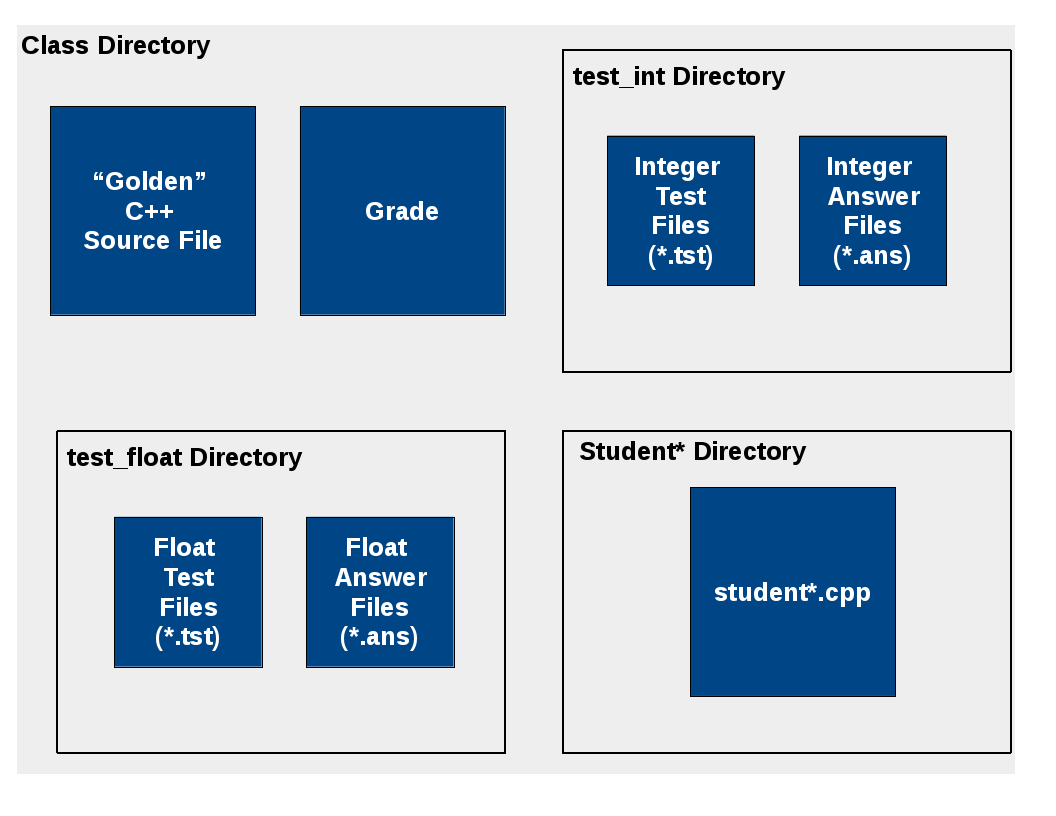
\includegraphics[width=0.6\textwidth]{./directorylayout}
\end{center}
\caption{Directory Layout \label{directorylayout}}
\end{figure}


\section{System  Versioning Information}
Major release versions:
\begin{itemize}
	\item Version 1.0.0 - {\it Cookies-n-Cream}
	\item Version 2.0.0 - {\it Dulce De Leche}
	\item Version 3.0.0 - {\it Rocky Road}
\end{itemize}
